\documentclass[16pt,a4paper]{article}
\usepackage[utf8]{inputenc}
\usepackage{amsmath}
\usepackage{amsfonts}
\usepackage{amssymb}
\usepackage{amsthm}
\usepackage{physics}



\usepackage[many]{tcolorbox}
\tcbuselibrary{skins,breakable}
\usepackage{hyperref}
\usepackage{mathtools}
\DeclarePairedDelimiter\ceil{\lceil}{\rceil}
\DeclarePairedDelimiter\floor{\lfloor}{\rfloor}

\hypersetup{
    colorlinks=true,
    linkcolor=blue,
    filecolor=magenta,      
    urlcolor=cyan,
    bookmarks=true,
    pdfauthor=Thaqib,
    bookmarksopen=true
}

\newtcbtheorem{defn}{Definition}{
    width=\textwidth,
    colback=white!20,
    colframe=orange,
    colbacktitle=orange,
    fonttitle=\bfseries,
    sharp corners,
    boxrule=1pt,
    breakable,
    enhanced,
    boxed title style={sharp corners},
    attach boxed title to top left
}{def}


\newtcbtheorem{axm}{Axiom}{
    width=\textwidth,
    colback=white!20,
    colframe=black,
    colbacktitle=black,
    fonttitle=\bfseries,
    sharp corners,
    boxrule=1pt,
    breakable,
    enhanced jigsaw,
    boxed title style={sharp corners},
    attach boxed title to top left
}{axm}

\newtcbtheorem{prop}{Proposition}{
    width=\textwidth,
    colback=white!20,
    colframe=black,
    colbacktitle=black,
    fonttitle=\bfseries,
    sharp corners,
    boxrule=1pt,
    breakable,
    enhanced jigsaw,
    boxed title style={sharp corners},
    attach boxed title to top left
}{prop}

\newtcbtheorem{thm}{Theorem}{
    width=\textwidth,
    colback=deepblue!2,
    colframe=deepblue,
    colbacktitle=deepblue,
    fonttitle=\bfseries,
    sharp corners,
    boxrule=1pt,
    breakable,
    enhanced,
    boxed title style={sharp corners},
    attach boxed title to top left
}{thm}

\newtcbtheorem{lemm}{Lemma}{
    width=\textwidth,
    colback=deepred!0,
    colframe=deepred,
    colbacktitle=deepred,
    fonttitle=\bfseries,
    sharp corners,
    boxrule=1pt,
    breakable,
    enhanced,
    boxed title style={sharp corners},
    attach boxed title to top left
}{lemm}



\newtcbtheorem{coll}{Corollary}{
    width=\textwidth,
    colback=white!20,
    colframe=dkgreen,
    colbacktitle=dkgreen,
    fonttitle=\bfseries,
    sharp corners,
    boxrule=1pt,
    breakable,
    enhanced,
    boxed title style={sharp corners},
    attach boxed title to top left
}{thm}




\usepackage{setspace}
\setstretch{1.7}
\usepackage{graphicx}
\usepackage[left=2cm,right=2cm,top=2cm,bottom=2cm]{geometry}

\usepackage{listings}
\usepackage{color}
\definecolor{dkgreen}{rgb}{0,0.3,0}
\definecolor{gray}{rgb}{0.5,0.5,0.5}
\definecolor{mauve}{rgb}{0.58,0,0.82}

\definecolor{deepblue}{rgb}{0,0,0.5}
\definecolor{deepred}{rgb}{0.6,0,0}
\definecolor{deepgreen}{rgb}{0,0.5,0}
\lstset{frame=tb,
  language=python,
  aboveskip=2mm,
  belowskip=2mm,
  showstringspaces=false,
  columns=flexible,
  basicstyle={\linespread{0.9}\small	tfamily},
  numbers=none,
  numberstyle=	iny\color{gray},
  keywordstyle=\color{blue},
  commentstyle=\color{dkgreen},
  stringstyle=\color{deepred},
  breaklines=true,
  breakatwhitespace=true,
  tabsize=4
}

\theoremstyle{definition}
\newtheorem{definition}{Definition}[section]

\newtheorem{theorem}{Theorem}[section]
\newtheorem{corollary}{Corollary}[theorem]
\newtheorem{lemma}[theorem]{Lemma}


\newcommand{\ang}[1]{\langle #1 \rangle}

\newcommand{\OR}{\vee}

\newcommand{\AND}{\wedge}

\author{Thaqib Mo.}
\title{ Reading-18 Groups }
\begin{document}
\maketitle
\newpage




\section{Binary operators}

\begin{defn}{Binary operation}{}
Let $S$ be a set. A binary operator on $S$ is a function from $S\times S$ to $S$. If $*: S\times S \rightarrow S$. For any 2 $a,b\in S$ we write $a*b$ to denote $*(a,b)$
\end{defn}
\begin{figure}[hbtp]
\centering
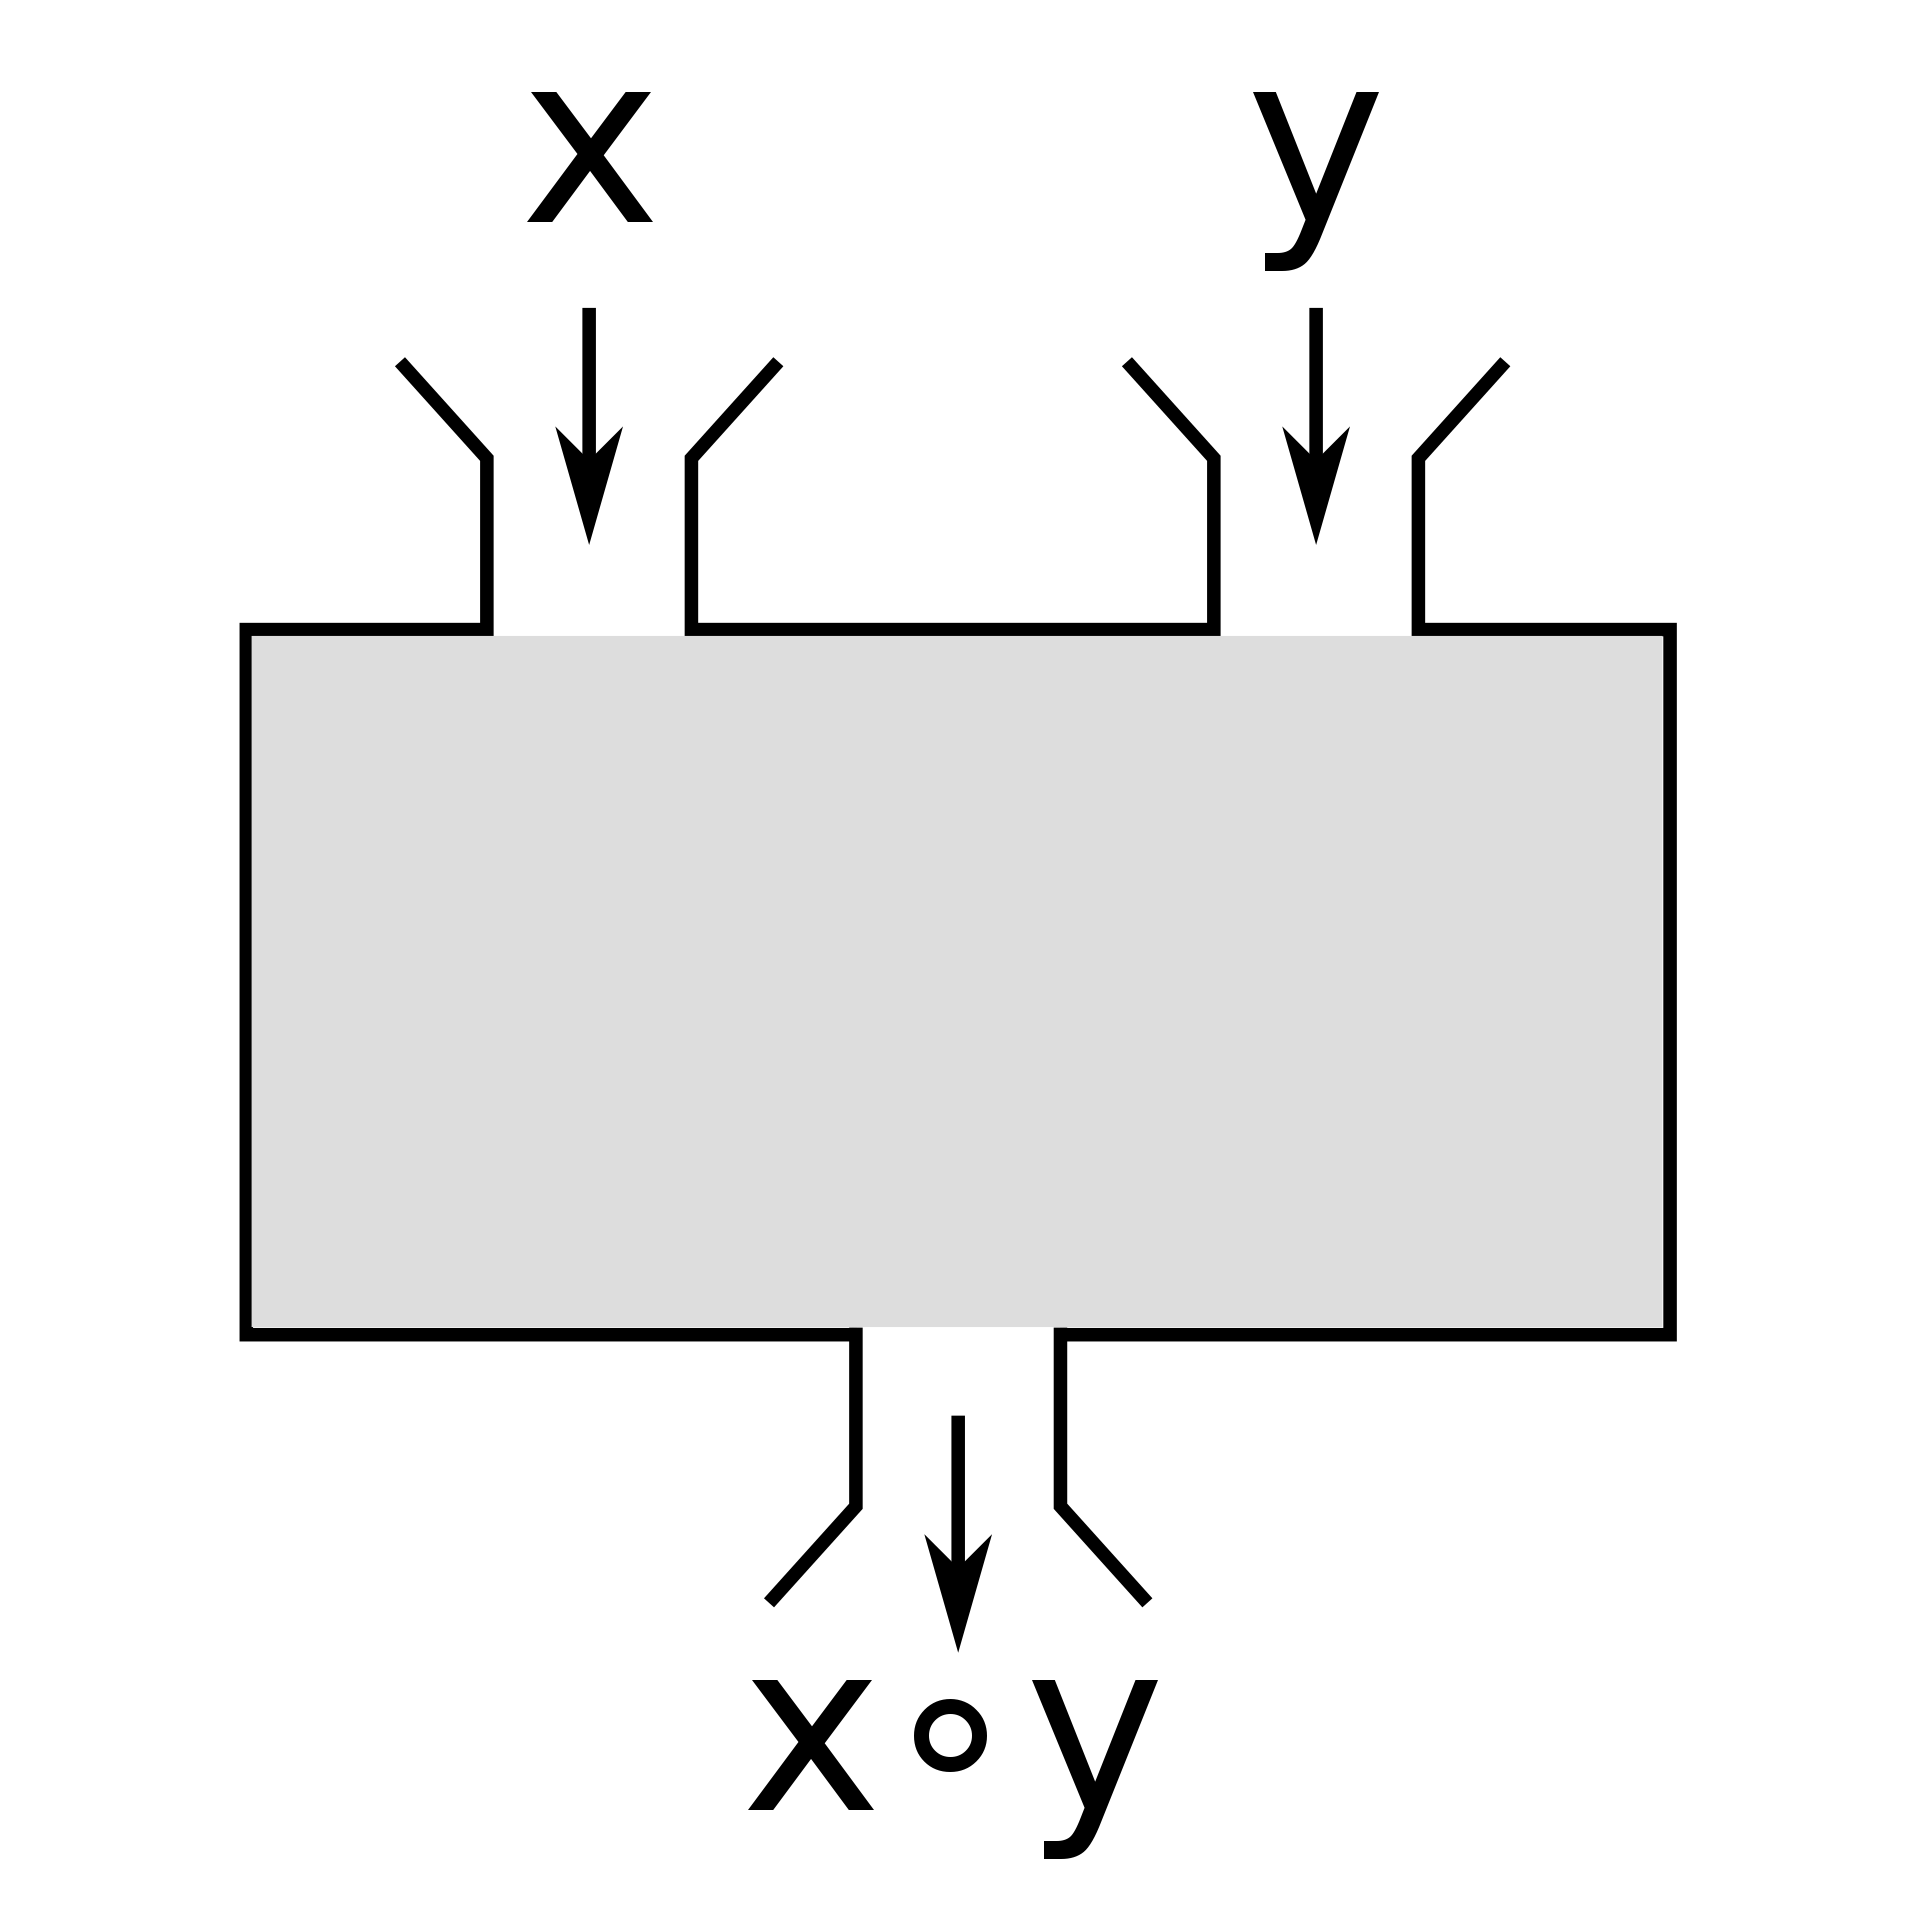
\includegraphics[scale=0.1]{figs/fig1.png}
\end{figure}

Some examples of binary relations are:

\begin{itemize}

\item[Example 1] On the set $\mathbb{Z}$, the operations $+,-,\times$ all are binary operations. Division is not a binary operator on $\mathbb{Z}$ since it can output a number outside $\mathbb{Z}$. 

\item[Example 2] For any set $A$, the operations $\cup, \cap$ define binary operations on $\mathcal{P}(A)$, giving ways of taking pairs of subsets of $A$ and defining new sets.  


\end{itemize}


\begin{defn}{Types of Binary operators}{}
\begin{itemize}
\item[\#] Let $S$ be a set and let $*$ be a binary operation on $S$. The binary operation is \textbf{associative} if for $a,b,c \in S$ we have $(a*b)*c = a*(b*c)$   





\item[\#] Binary operation  $*$ is \textbf{commutative} if for all $a,b \in S$ we have $a*b = b*a$. 

\item[\#] The element $e\in S$ is said to be \textit{unit} or \textit{identity} element if $a*e = e*a = a$ for all $a\in S$ 






\end{itemize}
\end{defn}



Associative property is very powerful because it the way we bracket the operations does not matter $(a*b)*(c*d) = (a*b*c)*d$ and many other ways. This can be formally proved.  

\begin{prop}{}{}
Let $S$ be a set with a associative binary relation $*$. If $a_1, a_2, a_3,\ldots a_n$ with $n\geq 1$ are elements of $S$ then the product 
\[a_1 * a_2 * a_3 * \cdots * a_n\]
is well defined, regardless the choice of bracketing. 
\end{prop}


\begin{proof}
Notation:\\
We define recursively $\langle a_1 \rangle = a_1$, $\langle a_1, a_2\rangle = a_1*a_2$, and for $n\geq 3$ we have 
\[\langle a_1, a_2, a_3, \ldots, a_n\rangle = \langle a_1, a_2, a_3, \ldots, a_{n-1}\rangle*a_n\] 

We prove by strong induction on $n$ that every product on $n$ elements is equal to the standard product. Since there is no choice of bracketing on $n=1$ and $n=2$ those cases hold true. Now assume that $P(n)$ is true upto $n$, where $n\geq 2$. Now consider $P(n+1)$. The product $a_1*a_2*a_3*\cdots *a_n * a_{n+1}$ can be expressed as $b*c$ which is the last application of $*$. \\
Where $b$ is the product of some elements $a_1, a_2, a_3, \ldots a_k$ and $c$ is the rest $a_{k+1}, a_{k+2}, \ldots a_{n+1}$. \\

If we have $k=n$, then $c=a_{n+1}$, by inductive hypothesis $b=\langle a_1, a_2, \ldots, a_n\rangle$ is well defined. So we have $b*c = \langle a_1, a_2, \ldots, a_n\rangle * a_{n+1} = \langle a_1, a_2, \ldots, a_n, a_{n+1}\rangle$ by definition of the standard product. Otherwise if $k<n$, then $c=\langle a_{k+1}, a_{k+2}, \ldots, a_{n+1}\rangle = \langle a_{k+1}, a_{k+2}, \ldots, a_{n}\rangle  *a_{n+1}$ and we have $b=\langle a_1, a_2, a_3, \ldots, a_k \rangle$. 

\[b*c = \langle a_1, a_2, a_3, \ldots, a_k \rangle * (\langle a_{k+1}, a_{k+2}, \ldots, a_{n}\rangle  *a_{n+1})\]
\[=(\langle a_1, a_2, a_3, \ldots, a_k \rangle * \langle a_{k+1}, a_{k+2}, \ldots, a_{n}\rangle)  *a_{n+1}\]
\[=\langle \langle a_1, a_2, a_3, \ldots, a_n \rangle *a_{n+1} = \langle a_1, a_2, a_3, \ldots, a_{n+1}\rangle \]


\end{proof}
\begin{figure}[hbtp]
\centering
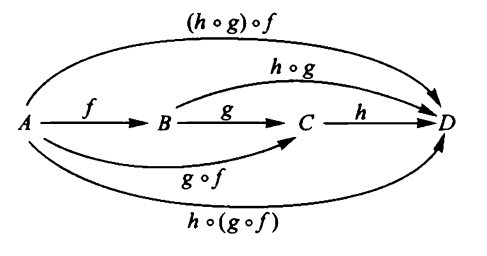
\includegraphics[scale=1]{figs/fig2.png}
\end{figure}


\section{Monoids, Inverse Elements, and Groups}

\begin{defn}{Monoid}{}
Let $S$ be a set with operation $*$. We call $S$ a \textit{monoid} if the operation $*$ is associative and has identity element $e\in S$ with respect to $*$.   
\end{defn}

\begin{thm}{Uniqueness of identity for monoids}{}
The identity element of a monoid is unique. 
\end{thm}
\begin{proof}
Let $S$ be a monoid. Suppose $S$ has 2 identity elements, $e_1, e_2 \in S$ for any $a\in S$ we know that $e_1a = ae_1 = a$ and $e_2a= ae_2 = a$. Using $a=e_1$ for the first equality $e_1e_2 = e_2e_1 = e_2$ and applying the second with $a=e_1$ we get $e_2e_1= e_1e_2 = e_1$. Therefore we have $e_1 = e_2$. 
\end{proof}


\begin{defn}{Unit}{}
Let $S$ be a monoid. An element $a\in S$ is called \textit{unit} if there exits some $b\in S$ such that $ab=ba=e$ where $e$ is the identity element. If this is the case we call $b$ the \textit{inverse} of $a$. 
\end{defn}

\begin{lemm}{Uniqueness of inverse of any unit}{}\label{uniq-inv}
In any monoid, the inverse of any unit is unique.
\end{lemm}
\begin{proof}
Let $S$ be a monoid, let $a$ be a unit. Suppose $b_1$ and $b_2$ are both inverse. Then $b_1a=ab_1=e$ and $b_2a=ab_2 = e$. By definition of the identity element 
\[b_1 = b_1e = b_1(b_2a)=(b_1a)b_2 = eb_2 = b_2\]
\end{proof}


\newpage
\section{Groups}
Now we can define groups.
\begin{defn}{Groups}{}
A set $G$ with the binary operation $*$ is a group if $G$ is a \textit{monoid} and every element in $G$ is a \textit{unit}. If $*$ is also commutative then $G$ is called an \textit{abelian group.}
\\
So a set $G$ with operation is called a \textit{group} if:
\begin{itemize}
\item[\# 1] For all $a,b,c\in G$ we have $a(bc) = (ab)c$. (Associativity). 

\item[\# 2] There is some $e\in G$ such that $ae=ea=a$ for all $a\in G$. (Identity)

\item[\# 3] For all $a\in G$, there is $b\in G$ such that $ab=ba=e$. (Inverse). 

\item If $G$ is an abelian group the optional 4th condition applies.  

\item[\# 4] For all $a,b \in G$ we have $ab = ba$. (Commutative). 
\end{itemize}
\end{defn}
Some examples of groups. 
\begin{itemize} 
\item[Example 1] The set $\mathbb{Z}$ with the operation $+$ is an abelian group. $0$ is the identity element and $-a$ is the inverse of any element $a$. Similarly the set $\{1,-1\}$ of units in $\mathbb{Z}$ with respect to the multiplication operation $\times$ is an example of finite abelian group.   
\end{itemize}

\begin{thm}{}{}
Let $M$ be a monoid and let $M^*$ be the units of $M$, then $M^*$ is a group called the group of units of $M$
\end{thm}
\begin{proof}
(Closed) Assume we have $a,b\in M^*$, we know that $a^{-1}, b^{-1} \in M^*$, by definition, $aa^{-1}=a^{-1}a=e=bb^{-1}=b^{-1}b$. Then get have 

\[(ab)(b^{-1}a^{-1}) = aea^{-1} = aa^{-1}=e\]
\[(b^{-1}a^{-1})(ab) = beb^{-1} = bb^{-1}=e\]
This shows that $ab$ has an inverse $(ab)^{-1}=a^{-1}b^{-1}$. So $M^*$ is closed. \\

Associativity, and Inverse is trivial by construction of $M^*$ and the identity element $e\in M$ is its own inverse so $ee = e$ therefore we have $e\in M^*$. 



 
\end{proof}

\newpage


\subsection{Exponent notation for Groups}

For a group $G$ and $g\in G$ we set $g^0 = e$ the identity element, $g^1 =g$ and $g^m$ to be the product of $m$ copies of $g$. 

\[g^m = \underbrace{ggg\cdots ggg}_{\text{$m$ coppies}}\]


\begin{thm}{}{}
Let $G$ be a group and $g,h\in G$
\begin{itemize}
\item[(1)] For all $n,m \in \mathbb{Z}$ we have $g^{n+m} = g^n g^m$
\item[(2)] For all $n,m \in \mathbb{Z}$ $(g^n)^m = g^{mn}$
\item[(3)] If $g$ and $h$ commute ($gh = hg$) then $(gh)^n = g^nh^n$

\end{itemize}
\end{thm}

\begin{proof}
By induction on $n$
\begin{itemize}
\item[(1)] $P(0)$ $g^{0+m} = g^0 g^m = eg^m = g^m$ base case holds. Assume $P(n)$ is true. Now consider $P(n+1)$

\[g^{n+1}g^m = (g\cdot g^n)\cdot g^m = g\cdot (g^n \cdot g^m)= g\cdot g^{n+m}\]

If $n+m\geq 0$ then the result is multiplying $m+n$ copies of $g$ with one more copy which is $g^{m+n+1}$ by definition. If $m+n=-1$ then $gg^{-1}=e$ which is $g^{1-1}=0$. Finally if $n+m\leq 2$ then it is multiplying $|m+n|$ copies of $g^{-1}$ and one copy of $g$, which is $|n+m|-1$ copies of $g^{-1}$. Thus $(1)$ holds for all $n\in \mathbb{N}$ and $m\in \mathbb{Z}$ applying the same argument for $m\in \mathbb{N}$ and $n\in \mathbb{Z}$ proves $(1)$. $\blacksquare$


\item[(2)] For $n=0$ we have $(g^m)^0 = e$, and $g^{0\times m} = g^0 = e$. Now assume it holds for some $n$. Consider $n+1$, we can apply (1)

\[(g^m)^{n+1} = (g^m)^n\cdot g^m = g^{mn}\cdot g^m = g^{m(n+1)}\]
If $n$ is a negative integer let $n=-l$ then $(g^m)^n = (g^m)^{-l} $. For any $h\in G$, $h^{-l}$ is product of $h^{-1}$ $l$ times. So we have 

\[(g^m)^{-l} = ((g^m)^l)^{-1} = (g^{ml})^{-1} = g^{-ml} = g^{m(-l)} = g^{mn} \qquad \blacksquare\] 





\newpage
\item[(3)] For $n=0$ we have $(gh)^0 = e = ee  = g^0h^0$, so base case holds true. Assume (3) holds for some $n$ and Now consider $P(n+1)$

\[(gh)^{n+1} = (gh)^n (gh) = g^n(h^ng)h= (g^ng)(h^nh) = g^{n+1}\cdot h^{n+1} \]
If $n$ is in the form $n=-l$ for some $l\in \mathbb{N}$ we get
$$(gh)^n = (gh)^{-l} = ((gh)^l)^{-1} = (g^lh^l)^-1 = h^{-l}g^{-l} = h^ng^n = g^nh^n$$


\end{itemize}
\end{proof}


\section{Orders of Elements and Cyclic Groups}

\begin{thm}{}{}
Let $G$ be a group and let $g\in G$ be an element. Then 
\[\ang{g} = \{g^k : k\in \mathbb{Z}\} \text{ is a group}\]

\end{thm}
\begin{proof}
Closure, for any $g^m, g^n \in \ang{g}$ consider $g^m\cdot g^n$ by the above theorem we have $g^m\cdot g^n = g^{m+n} \in \ang{g}$. Associative is automatic since $G$ is a group. We have $g^0 = e$ by definition so we have $g^0 \in \ang{g}$ therefore the identity property is also satisfied. Finally for any $g^m \in \ang{g}$ we also have $g^{-m} \in \ang{g}$ so the inverse property is also satisfied. Therefore $\ang{g}$ is a group. 
\end{proof}


\begin{defn}{Cyclic Group}{}
If $g\in G$ is an element , the set $\ang{g}$ is a subgroup of $G$ generated by $g$. If $G = \and{g}$ for some element in $g$ we say that $G$ is a \textit{cyclic group} and that $g$ is a \textit{generator} of $G$. 
\end{defn}
\begin{figure}[hbtp]
\centering
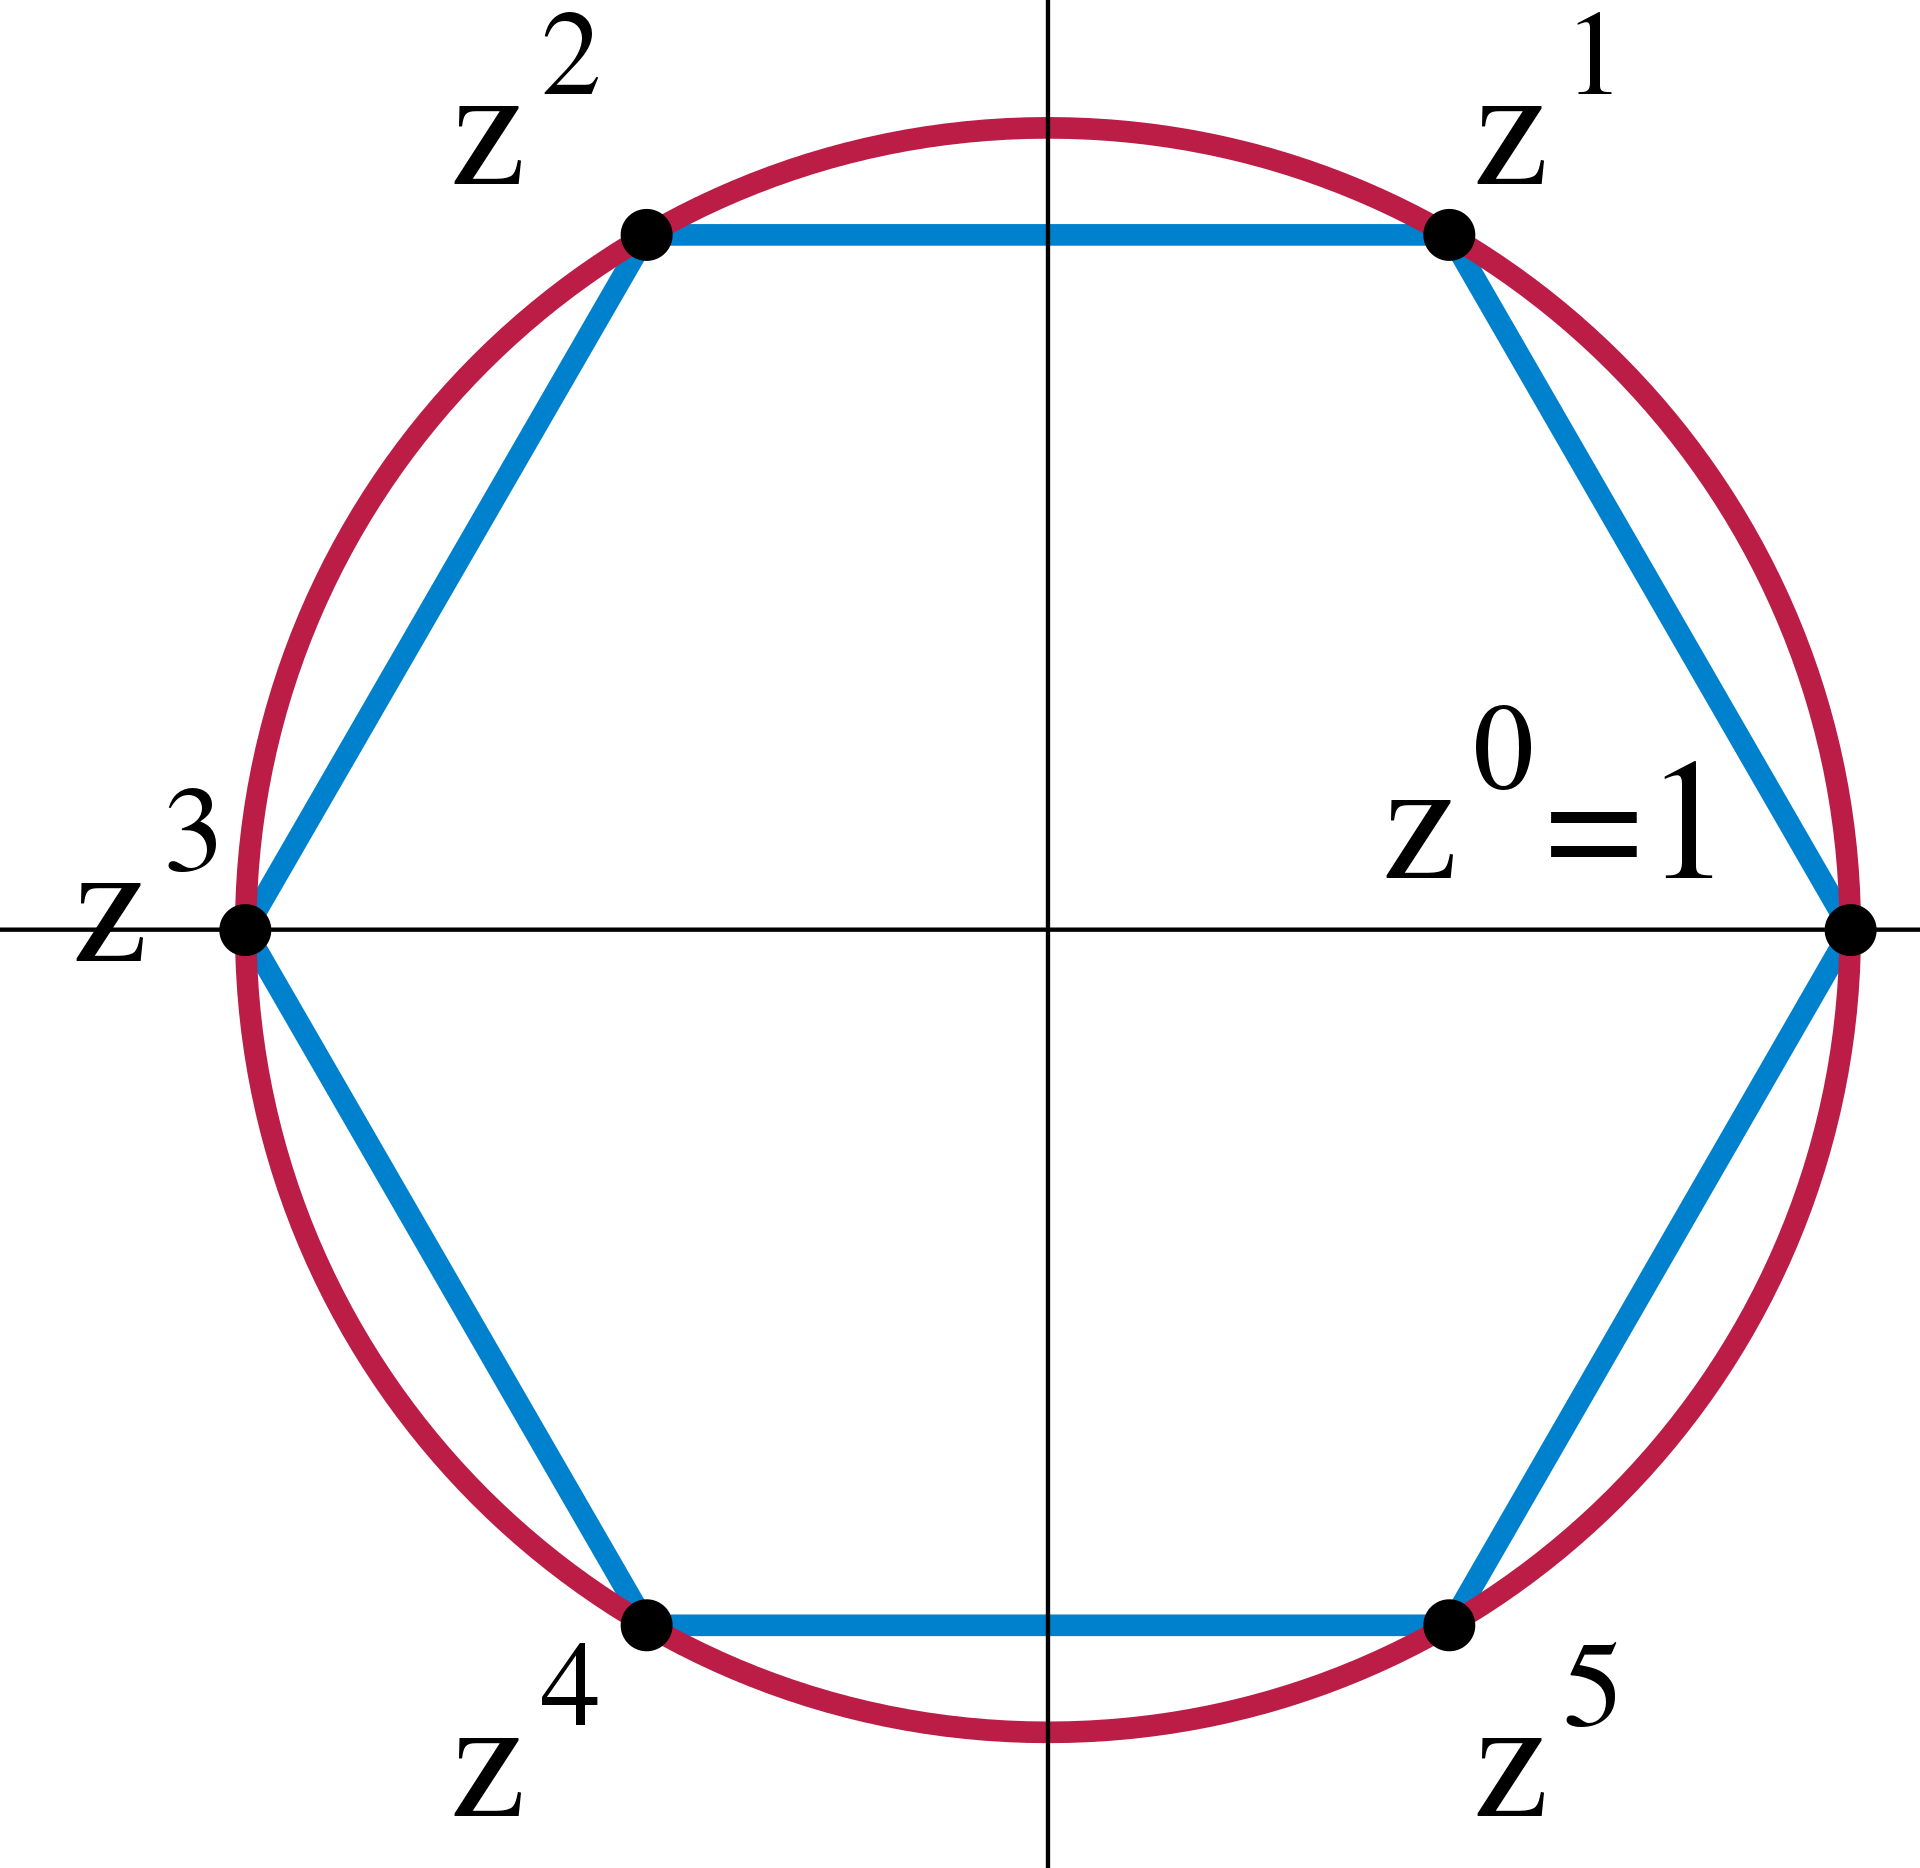
\includegraphics[scale=0.1]{figs/fig3.png}
\end{figure}


\paragraph{Example} The set of integers modulo $n$. This is denoted by $\mathbb{Z/}n\mathbb{Z}$ where $n$ is a positive integer. To define the group we take the set of equivalence classes of $\mathbb{Z}$ under the modulo relation. Which is defined as follows

\[a\equiv b \; (\bmod n) \text{ if $n | a-b$}\]

Here $n|a-b$ means $n$ divides $a-b$, if there is some $k\in \mathbb{Z}$ such that $a-b = kn$. The equivalence classes are $[0], [1], [2], \ldots [n-1]$. The addition can be defined via:

\[[a]+[b] = [a+b]\]\label{pg6}
For any $a,b \in \mathbb{Z}$. We can prove this is well defined and the identity element is $[0]$ and inverse of $[a]$ is $[-a]$. We can show that this forms a \textit{finite abelian group}.  

\begin{defn}{Order}{}
Given any group $G$ and element $g\in G$, the order of $g$ denoted by $o(g)$ is the smallest integer $n\geq 1$ such that $g^n = e$, if such integer exists. Otherwise if $g^n\neq e$ for any $n\geq 1$ we write $o(g) = \infty$ 
\end{defn}

\begin{prop}{}{}
For a group $G$ and $g\in G$ we have $o(g) = o(g^{-1})$
\end{prop}

\begin{proof}
If we have $o(g) = \infty$ then we have no integer $n\geq 1$ such that $g^n = e$ taking the inverse on both sides $(g^{-1})^n\neq e$ so $o(g^{-1}) = \infty$. Otherwise if we have $o(g) = n$ for some $n\geq 1$. Then we have 
\[g^n = e\]
Taking the inverse of both sides $g^{-n} = e^{-1} = (g^{-1})^n = e$. Now assume there is some $m<n$ such that $g^{-m} = e$ again taking the inverse of both sides $g^m = e^{-1} = e$ which contradicts the definition of $o(g)$.  
\end{proof}



\begin{thm}{}{}\label{thm5}
Let $G$ be a group and let $g\in G$ be an element of finite order $n$. Then:

\begin{itemize}
\item[(1)] $g^k = g^m$ if and only if $k\equiv m \bmod n$
\item[(2)] We have $\ang{g} = \{e,g,g^2, \ldots g^{n-1}\}$, In particular the size of $\ang{g}$ is $o(g)$. 
\end{itemize}
\end{thm}
\begin{proof}
Suppose $k \equiv m\bmod n$ for some $k,m\in \mathbb{Z}$. By definition we have $k-m = \ell n$ for some $\ell \in \mathbb{Z}$. Since $g^n = e$ we also have $g^{\ell n} = e^\ell = e$. Therefore $g^{k-m} = e$. Multiplying by $g^m$ gives $g^k = g^m$.  Conversely suppose $g^k = g^m$. This implies $g^{k-m} = e$. To show that $n|k-m$, consider the division with remainder. We have
\[k-m = nq + r\] 
But then $$e=g^{k-m}=g^{nq+r} = g^{nq}\cdot g^r = e^qg^r = g^r$$. Since $r<n$ the definition of $o(g)$ forces $r=0$ therefore we have $k-m = qn$ and $k=m\bmod n$. Thus $g^k = g^m$. 
\\

To prove $(2)$ we clearly have $\{e, g, g^2, \ldots g^{n-1}\} \subseteq \ang{g}$. In the other direction suppose $k\in \mathbb{Z}$, and using division by remainder to write $k=nq+r$ we have shown $g^k = g^r$ and we must have $0\leq n < r$ which shows $g^k \subseteq \{e,g,g^2, \ldots, g^{n-1}\}$. So we have $\ang{g} = \{e,g,g^2, \ldots g^{n-1}\}$
\end{proof}





\newpage

\section{Subgroups}

\begin{defn}{Subgroups}{}
If $(G,\ast)$ is a group then $H\subset G$ is a subgroup if $(H,\ast)$ itself is also a group. 
\end{defn}
The first example is the trivial subgroup for any group, which is $\{e\}$ just the identity element. Other examples are $\mathbb{Z}$ is a subgroup of $\mathbb{Q}$ under addition and $\mathbb{Q}$ is a subgroup of $\mathbb{R}$ under addition. 

\begin{thm}{Subgroup Test}{}
Let $G$ be a group and let $H$ be a non empty subset of $G$. Then $H$ is a subgroup of $G$ if and only if for all $a,b\in H$ we have $ab^{-1}\in H$
\end{thm}\label{test}


\begin{proof}

Suppose $H$ is a subgroup of $G$. For each $a,b\in H$ we know that $b^{-1}\in H$ since $H$ is a group. Then since $H$ is closed with respect to the operation we get $a\cdot b \in H$. \\

Conversely, suppose that for all $a,b \in H$ we have $ab^{-1}\in H$. Since $H$ is non empty taking $a=b$ we get $aa^{-1}\in H$ so the identity element is in $H$. Let $b\in H$ and let $a=e$ then $eb^{-1}=b^{-1}\in H$ so for any $b\in H$ its inverse is also in $H$. The operation is associative automatically. To see the operation is closed  we know that $b^{-1}\in H$ and so $a({b^{-1}})^{-1}=ab\in H$. 
\\

If we let $e_H$ to be the identity of $H$ and $e_G$ to be the identity of $G$, then we have shown that $e_G\in H$ and by uniqueness of identity we have $e_G = e_H$.  Similarly let $h\in H$ we have shown that $h^{-1}$ its inverse in $G$ also belongs to $H$. So $h$ has inverse in $H$. By \hyperref[uniq-inv]{uniqueness of inverse} the inverse of $h$ in $G$ and $H$ is same.   
\end{proof}

\subsection{Examples of Subgroup test}
\subsubsection*{Example 1 (Center of a group)} Let $G$ be a group. We define the \textit{\textbf{center}} of the group to be: 

\[Z(G) = \{z\in G : zg = gz \text{ for all $g\in G$}\}\]

We can verify that $Z(G)$ is an abelian group. First $e\in Z(G)$ since $eg = ge= g$ . Now suppose $a,b \in Z(G)$. We must verify $ab^{-1}\in Z(G)$. Now assume we have some $b\in Z(G)$ then $gb=bg$ applying $b^{-1}$ on both sides 
\[b^{-1}gbb^{-1} = b^{-1}bgb^{-1}\]
\[b^{-1}g = gb^{-1}\]
Therefore $b^{-1} \in Z(G)$, now 
\[(ab^{-1})g = a(b^{-1}g) = (ag)b^{-1} = (ga)b^{-1} = g(ab^{-1})\]
Hence we have $ab^{-1}\in Z(G)$ therefore $Z(G)$ is an subgroup. To see why it is abelian, consider $a,b\in Z(G)$ then assume we have $a,b \in Z(G)$ then we also have $ab\in Z(G)$ since we know that $ag=ga$ then set $g=b$ to get $ab=ba$ hence $Z(G)$ is commutative. 


\subsubsection*{Example 2 Conjugate}\label{cong}
Suppose $H$ is a subgroup of $G$, and for $g\in G$ we define the conjugate of $H$ in $G$ by $g$ to be

\[gHg^{-1} = \{ghg^{-1} : h \in H\}\]
We know that $gHg^{-1}$ is empty because $H$ is non empty. So let $a,b \in gHg^{-1}$ then $a=gh_1g^{-1}$ and $b=gh_2g^{-1}$ for $h_1, h_2 \in H$. 

\begin{align*}
ab^{-1} =gh_1g^{-1} (gh_2g^{-1})^{-1}\\
= gh_1g^{-1} (gh_2^{-1}g^{-1})\\
=gh_1h_2^{-1}g^{-1}
\end{align*}

Since $h_1h_2^{-1}\in H$ by definition of the group we have $ab^{-1}\in gHg^{-1}$ so it is a group by the subgroup test. 


\subsubsection*{Example 3}
Let $C_4$ be the cyclic group with $4$ elements. $C_4 = \{e,a,a^2, a^3\}$. The trivial subgroup $\{e\}$ is obviously a subgroup. If we construct a subgroup $H$, assume we have $a\in H$ then we must have $a^{-1}=a^3\in H$ and similarly we should also have $a\cdot a = a^2 \in H$, and we must also have the identity so $H=C_4$. So $H$ is not a proper subgroup of $C_4$, it is the similar case if we start with $a^3$, but if we start with $a^2$, assume $a^2 \in H$ then we must also have $e\in H$ and $(a^2)^{-1} = a^{-2}=a^4 = e$ so $H=\{e,a^2\}$ is a subgroup of $C_4$. Only the trivial subgroup and $\{e,a^2\}$ are subgroups of $C_4$. 
\newpage
\section{Symmetric Groups}
The set of bijections from a set $A$ to it self is a group, with compositions ($\circ$) as the group operation. If we restrict $A$ to a finite set that means we have $|A| = n$ Here we can treat the bijections from $A\rightarrow A$ as the set of bijections from $\{1,2,3,\ldots n\}$ to itself. This is denoted by $S_n$ and it is called the \emph{Symmetric group of degree $n$}. We can represent the elements of this group using a matrix. 
\\
It is an matrix with 2 rows with the top row containing the numbers $1,2,\ldots n$ and for $\sigma \in S_n$ the bottom row contains $\sigma(1), \sigma(2)\ldots$. For example the identity element $\varepsilon$ with $\varepsilon(x)=x$ 
\begin{align*}
\varepsilon = 
\begin{pmatrix}
1 & 2 & 3 \quad\cdots \quad n \\
1 & 2 & 3 \quad \cdots \quad n
\end{pmatrix}
\end{align*}
Similarly a bijection $\tau$ that sends 1 to 2, 2 to 3 $\ldots n$ to 0 can be written as:

\begin{align*}
\tau = 
\begin{pmatrix}
1 & 2 & 3 \quad\cdots \quad n \\
2 & 3 & 4 \quad \cdots \quad 1
\end{pmatrix}
\end{align*}

\begin{prop}{Number of elements in symmetric groups}{}
$|S_n| = n!$
\end{prop}
For the first element we have $n$ choices and the next one we have $n-1$ then $n-2$ up until $1$ to the total number of choices is $n\times (n-1) \times \cdots \times 1 = n!$.  Another proposition that this leads to is: 

\begin{prop}{}{}
For $n\geq 3$ , the group $S_n$ is not non-abelian 
\end{prop} 

\begin{proof}
Assume for $n\geq 3$ , $S_n$ is abelian. We define 2 bijections: 
\begin{align*}
\tau = 
\begin{pmatrix}
1 & 2 & 3 \quad\cdots \quad n \\
3 & 2 & 1 \quad \cdots \quad n
\end{pmatrix} \quad\quad
\sigma = 
\begin{pmatrix}
1 & 2 & 3 \quad\cdots \quad n \\
2 & 1 & 3 \quad \cdots \quad n
\end{pmatrix}
\end{align*}
So $\sigma$ just swaps 1 and 2 and $\tau$ cycles through $1,2,3$. Both the bijections leave $4,5,6\ldots n$ fixed. So we have $(\sigma \circ \tau)(1) = \sigma (3) = 3$ but $(\tau\circ \sigma)(3) = \tau(3) = 1$ therefore we have $(\tau \circ \sigma)\neq (\sigma \circ \tau)$ therefore the group is non abelian. 
\end{proof}



\newpage
\section{Homomorphisms and Cosets}

\subsection{Group Homomorphisms}

\begin{defn}{Group Homomorphisms}{}
Let $G_1$ and $G_2$ be groups a function $\phi: G_1 \rightarrow G_2$ is called homomorphism if for all elements $a,b\in G_1$ we have 
\[\phi(ab) = \phi(a)\cdot \phi(b)\]
Here $\cdot$ is the binary operation in $G_2$
\end{defn}
\subsection*{Examples}
\subsubsection*{Example 1}
For any 2 groups there is always a homomorphism called the trivial homomorphism $\phi : G_1 \rightarrow G_2$ given by $\phi (a) = e_{G_2}$ for all $a\in G_1$ here $e_{G_2}$ is the identity element of $G_2$.  

\subsubsection*{Example 2}
For any positive integer $n$, the "Reduction modulo $n$" map $\phi : \mathbb{Z}\rightarrow \mathbb{Z/}n\mathbb{Z}$ defined by $\phi(m) = [m]$ is a homomorphism with respect to $+$ operation. 
\[\phi(m_1+m_2) = [m_1+m_2]\] 
From the example on \hyperref[pg6]{Page 6} we know that (by definition )
\[[m_1 + m_2] = [m_1]+[m_2]\]
Here the $+$ denotes different operations one is in $\mathbb{Z}$ and other one is in $\mathbb{Z/}n\mathbb{Z}$


\begin{thm}{Properties of Homomorphisms}{}
Let $\phi: G_1 \rightarrow G_2$ be a homomorphism. Then 
\begin{itemize}
\item[(1)] $\phi$ preserves the identity: $\phi(e_{G_1}) = e_{G_2}$
\item[(2)] $\phi$ preserves the inverse: $\phi(g^{-1}) = \phi(g)^{-1}$
\item[(3)] $\phi$ preserves the powers: $\phi(g^{m}) = \phi(g)^{m}$
\item[(4)] The composition of 2 homomorphisms,  $\psi : G_2\rightarrow G_3$ and $\phi : G_1 \rightarrow G_2$  then $\psi \circ \phi : G_1 \rightarrow G_3$ is also an homomorphism.  

\end{itemize} 
\end{thm}
\newpage
\begin{proof}
\begin{itemize}
\item[(1)] 
\[\phi(e_{G_1}) = \phi(e_{G_1}\cdot e_{G_1}) = \phi(e_{G_1}) \cdot \phi (e_{G_1})\]
Then \[\phi(e_{G_1})^{-1} \phi(e_{G_1}) = \phi(e_{G_1})^{-1} \phi(e_{G_1}) \cdot \phi (e_{G_1})\]
\[e_{G_2} = \phi(e_{G_1})\]


\item[(2)] For each $g\in G$ we have 
\[\phi(g)\phi(g^{-1}) = \phi(gg^{-1}) = \phi (e_{G_1}) = e_{G_2}\]
Similarly we have $\phi(g^{-1})\phi(g)=e_{G_2}$. By the uniqueness of inverse this shows that $\phi(g^{-1})=\phi(g)^{-1}$

\item[(3)] For $k=0$ we have $\phi(g^0) = \phi(e_{G_1}) = e_{G_2} = \phi(g)^0$. Now assuming it holds for some $k\in \mathbb{N}$, consider $k+1$

\[\phi(g^{k+1}) = \phi(g^k\cdot g) = \phi(g^k)\phi(g) = \phi(g)^k\phi(g) = \phi(g)^{k+1}\]
If $k<0$ then $k=-m$
\[\phi(g^{-m}) = \phi(g^{-1})^m = (\phi(g)^{-1})^m = \phi(g)^{-m}\]

\item[(4)] Consider $\psi\circ \phi(g\cdot h)$ We have $\psi(\phi(g)\cdot \phi(h)) = \psi(\phi(g))\cdot \psi(\phi(h))$ since $\phi$ and $\psi$ are both homomorphisms we by definition $\psi\circ \phi$ is also an homomorphism. 

\end{itemize}
\end{proof}


\begin{defn}{kernel}{}
If $\phi: G_1\rightarrow G_2$ is a homomorphism then the \textit{kernel} $\ker\phi$  is the set
\[\ker \phi = \{g\in G_1 : \phi(g) = e_{G_2}\}\]
\end{defn}
\begin{figure}[hbtp]
\centering
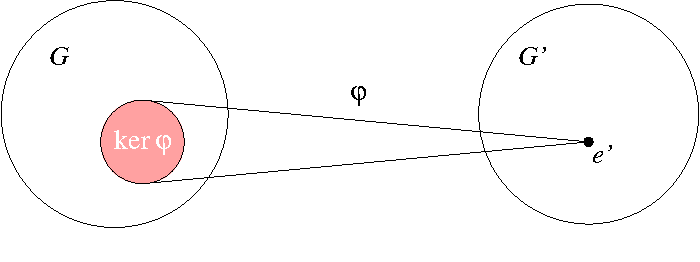
\includegraphics[scale=0.7]{figs/fig0.png}
\end{figure}


\begin{thm}{}{}
\begin{itemize}
\item[(1)] The set $\ker \psi$ is a subgroup of $G_1$
\item[(2)] The function $\psi$ is injective if and only if $\ker\psi = \{e_{G_1}\}$
\end{itemize}
\end{thm}
\begin{proof}
\begin{itemize}
\item[(1)] We can apply the subgroup test  from \hyperref[test]{Theorem 6}, First $\ker \phi$ is non empty because $e_{G_1}$ always belongs to the kernel. Now if $a,b\in \ker \phi$ then we need to show that $ab^{-1}\in \ker \phi$. Using the properties of homomorphisms 

\[\phi(ab^{-1}) = \phi(a)\phi(b^{-1}) = \phi(a)\phi(b)^{-1} = e_{G_2}\cdot e_{G_2} = e_{G_2}\]


\item[(2)] Suppose $\ker \phi$ is injective. Now suppose $g\in \ker \phi$ and let $\phi(g) = e_{G_2} = \phi(e_{G_1})$ since $\phi$ is injective we have $\phi = e_{G_2}$, so if $\phi$ is injective then $\ker \phi = \{e_{G_1}\}$. 
\\
Now assume that $\ker \phi = \{e_{G_1}\}$ suppose we have $a,b\in G_1$ such that $\phi(a) = \phi(b)$. 
\[\phi(b)^{-1}\phi(a) = \phi(b)\phi(b)^{-1} = e_{G_2}\]
The right hand side simplifies to $\phi(ab^{-1})$ since we have $ab^{-1}\in \ker\phi$ then $ab^{-1}=e_{G_1}$ this means we have $a=b$. Thus if $\ker\phi = \{e_{G_1}\}$ then $\phi$ is injective. 
\end{itemize}
\end{proof}
\subsection{Cosets}
We can describe equivalence classes on group elements using homomorphisms. If we have $\phi: G_1 \rightarrow G_2$, then let

\[H=\ker\phi\] 

Then for $a,b\in G$ we have $a\sim b$ if and only if $\phi(a) = \phi(b)$ but from the subgroup test we also know that $\phi(ab^{-1}) = e_{G_2}$ which is because we have $ab^{-1}\in H$. 
\\
This condition can be generalized to subgroups other than $\ker \phi$

\begin{thm}{}{}
Let $G$ be a group and let $H$ be a subgroup of $G$. We define the relation $\sim$ on $G$. We have $a\sim b$ if and only if $ab^{-1}\in H$. Then $\sim$ is an equivalence relation and the equivalence class of an element $a\in G$ is the set $Ha =\{ha : h\in H\}$ which is called the right coset of $H$ generated by $a$. 	
\end{thm}

\begin{proof}
$\quad$\\
\begin{itemize}
\item \textbf{Reflexive} For any $a\in G$ we have $a\sim a$ since $aa^{-1}=e\in H$ since $H$ is subgroup. 
\item \textbf{Symmetric} Assume we have $a\sim b$, so we have $ab^{-1}\in H$. Since $H$ is closed $(ab^{-1})^{-1} = ba^{-1}\in H$ which implies $b\sim a$. 

\item \textbf{Transitive} Assume we have $a\sim b$ and $b\sim c$ that means we have $ab^{-1}\in H$ and $bc^{-1}\in H$ since $H$ is closed 
\[ab^{-1}bc^{-1} = aec^{-1} = ac^{-1}\in H\]
Therefore we have $a\sim c$
\end{itemize}
This proves that $\sim$ is an equivalence relation. 
Now choose $a\in G$ by definition we have: 
\begin{align*}
[a] &= \{g\in G : g\sim a\}\\
&=\{g\in G : ga^{-1}\in H\} \\
&=\{g\in G : ga^{-1}\in H\} \\
&= \{g\in G : ga^{-1}=h \in H\}\\
&= \{g\in G : g=ha \in H\}\\
&= Ha
\end{align*}
This shows that the equivalence class of $[a]$ is the right coset generated by $a$. 
\end{proof}
We can define another relation $\sim_L$ with $a\sim_L b$ if $b^{-1}a\in H$, resulting in the equivalence class of the form $aH = \{ah : h\in H\}$ which is called the \textit{left coset} of $a$. If $G$ is abelian,then $aH=Ha$.   

\begin{figure}[hbtp]
\centering
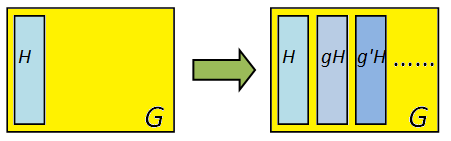
\includegraphics[scale=1]{figs/fig4.png}
\end{figure}
An important fact used for proving theorems involving costs is 

\begin{prop}{}{}
$Ha=Hb\iff ab^{-1}\in H$ 
\end{prop} 
\begin{proof}
$(\Rightarrow)$ Let $Ha=Hb$ then $a=hb$ for some $h\in H$ then applying $b^{-1}$ leads to $ab^{-1}=h\in H$. For the $(\Leftarrow)$ part assume we have $ab^{-1}\in H$. Then $ab^{-1}=h\leadsto a=hb \leadsto a\in Hb \Rightarrow Ha=Hb$ (Since $a$ is arbitrary and the argument is symmetric in $a,b$).
\end{proof}

\subsubsection*{Example}
 Let $G= \mathbb{Z}$. Let $n$ be a positive integer, the set 
 \[H=n\mathbb{Z} = \{m\in \mathbb{Z} : m=nk \text{ for some $k\in \mathbb{Z}$}\}\]
This is a subgroup of $\mathbb{Z}$. Since the group operation is $+$ we can define the cosets as $n\mathbb{Z} + a$. Moreover, if we have $b\in n\mathbb{Z}+a$ if and only if $b\sim a$ this holds true if $b-a\in n\mathbb{Z}$ this is same as $n|(b-a)$ so $b$ belongs to the equivalence class of $[a] = n\mathbb{Z}+a$ if and only if $b\equiv a\bmod n$, thus this equivalence class here is the equivalence class of congruence modulo $n$ 


\section{Normal Subgroups and Quotient Groups}
\begin{defn}{Normal Subgroup}{}
Let $G$ be a group, a subgroup $H$ is called a \emph{normal} subgroup if $gHg^{-1}=H$ defined by 
\[gHg^{-1} = \{ghg^{-1} : h \in H\}\]
In this case the notation $H\lhd G$ is used to denote that $H$ is a normal subgroup of $G$. 
\end{defn}
The conjugate subgroup shown to be a sub group in in \hyperref[cong]{Example 2}. If $G$ is abelian then we have the following: 

\begin{prop}{}{}
Every subgroup of an abelian group is normal. 
\end{prop}
\begin{proof}
Consider a subgroup $H$ of $G$ an abelian group. Now for any $h\in H$ consider 
\[ghg^{-1} = g(hg^{-1}) = (gg^{-1})h= eh = h\]
So we have 
\[gHg^{-1} = H\]
therefore $H$ is normal and we have, $H\lhd G$.  
\end{proof}
Another important theorem that follows is: 
\begin{thm}{}{}
Let $G$ be a group. For every subgroup $H$ of $G$ the product $(Ha)(Hb) = Hab$ is well defined multiplication of cosets if and only if $H\lhd G$. 
\end{thm}\label{well-def}
\begin{proof}
$(\Rightarrow)$ Let $(Ha)(Hb) = Hab$. Now consider some $h\in H$ and the cosets 
\begin{align*}
Hh = He \text{ and } Hg &= Hg\\
\leadsto (Hg)(Hh) &= (Hg)(He) \\
Hgh &= Hge \\
\text{ Since $H$ is a subgroup } &(gh)(ge)^{-1} \in H\Rightarrow ghg^{-1}\in H
\end{align*}
This proves that $gHg^{-1}\subseteq H$, taking $g^{-1}$ in place of $g$ above we get $g^{-1}Hg\subseteq H$. This directly implies $H\subseteq gHg^{-1}$
\\
$(\Leftarrow)$ Conversely, assume that $H\lhd G$. Suppose we have $a,b,a_1,b_1 \in G$ such that $Ha=Ha_1$ and $Hb=Hb_1$  then we have $aa_1^{-1} \in H $ and $bb_1^{-1}\in H$. We need to show $(Ha)(Hb)=(Ha_1)(Hb_1)$.  This is equivalent to $(ab)(a_1b_1)^{-1}\in H$. Then we have 
\[abb_1^{-1}a_1^{-1}=a(bb_1^{-1})a_1^{-1} = (a(bb_1^{-1})a^{-1})(aa_1^{-1})\]
Now, $aHa^{-1}=H$ and $bb_1^{-1}\in H $, so we have $(a(bb_1^{-1})a^{-1})\in aHa^{-1} = H$. Also $aa_1^{-1}\in H$ then we get that $(a(bb_1^{-1})a^{-1})(aa_1^{-1}) = a(bb_1^{-1})a_1^{-1}\in H$. Thus multiplication of right cosets is closed. 
\end{proof}

Some important properties of subgroups are: 

\begin{thm}{Properties of Quotient groups}{}
Let $G$ be a group and $H\lhd G$ then
\begin{itemize}
\item[(1)] The set $G/H$ if right costs of $H$ is a group under the operation $(Ha)(Hb) = Hab$ called the \emph{quotient} group of $G$ by $H$.  

\item[(2)] The function $\phi : G\rightarrow G/H$ given by $\phi(g) = Hg$ is a surjective homomorphism, called the \emph{quotient mapping}. 

\item[(3)] If $G$ is abelian, then $G/H$ is abelian. 

\item[(4)] If $G$ is cyclic then $G/H$ is cyclic. 

\end{itemize}
\end{thm} 
\begin{proof}
\begin{itemize}
\item[(1)] \hyperref[well-def]{Theorem 10} tells us that the the operation is well defined when $H$ is normal. For associativity consider 
\[((Ha)(Hb))(Hc) = (Hab)(Hc) = H(ab)c = Ha(bc) = (Ha)(Hbc) = (Ha)((Hb)(Hc))\]
The identity element is the coset $H=He$ and inverse of $Ha$ is $Ha^{-1}$. Thus $G/H$ is a group. 
\newpage
\item[(2)] Consider
 \[\phi(ab) = Hab = (Ha)(Hb) = \phi(a)\phi(b)\]
 Hence, $\phi$ is a homomorphism. For surjective,for any coset $Ha \in G/H$ we have $\phi(a) = Ha$. 

\item[(3)] If $G$ is abelian,then consider 
\[(Ha)(Hb) = Hab = Hba = (Hb)(Ha)\] 
 Hence the operation on $G/H$ is commutative. 
 
 \item[(4)] If we have $G=\ang{g}$ for some $g\in G$ then every element of $G$ is in the form $g^k$ for some $k\in \mathbb{Z}$, thus given $Ha\in G/H$ we know that $a=g^k$ for some $k\in \mathbb{Z}$. Then $Ha = Hg^k = \phi(g^k) = \phi(g)^k = (Hg)^{k}$ where $\phi$ is the quotient homomorphism. Since $\phi$ is surjective we have $G/H = \ang{Hg}$, so $G/H$ is also cyclic. 
\end{itemize}
\end{proof}
An example of quotient group is the group $\mathbb{Z}/n\mathbb{Z}$ it has elements in the form $n\mathbb{Z}+a$ which are the equivalence classes under the relation of congruence modulo $n$.
\\
\subsubsection*{Example} Consider the group $(\mathbb{Q},+)$, then $\mathbb{Z}$ is a group. Since $\mathbb{Q}$ is abelian, $\mathbb{Z}$ is automatically a subgroup. The elements of the quotient group $\mathbb{Q/Z}$ are of the form $\mathbb{Z}+q$ for $q\in \mathbb{Q}$.
\\
Every element of $\mathbb{Q/Z}$ has a unique representative of the form $\mathbb{Z} + \delta$ where $0\leq \delta \leq 1$. For any $q\in \mathbb{Q}$ we can round down $\mathbb{q}$ using the floor function  $\floor{q}$ then we have 
\[0\leq q-\floor{q}\leq 1\]
So we can set $\delta = q-\floor*{q}$. If we had $\delta^\prime$ such that $\delta + \mathbb{Z} = \delta^\prime \mathbb{Z}$ then $\delta - \delta^\prime \in \mathbb{Z}$. but due to the given constrains on $\delta$ we have $-1<\delta-\delta^\prime < 1$ the only integer is $0$ so we have $\delta=\delta^\prime$. 
\\
The group is countably infinite but every element has a finite order.  For any given coset $\mathbb{Z}+q$, we write $q=\frac ab$ where $a,b$ are integers and $b\neq 0$. Note that then $b(\mathbb{Z}+q) = \mathbb{Z}+bq = \mathbb{Z}+a=\mathbb{Z}+0$ So the order of the coset $\mathbb{Z}+\frac ab$ is at most $b$. 


\newpage

\section{Lagrange's Theorem}

An important definition is needed before the main theorem 

\begin{defn}{Index}{}
Let $G$ be a group and let $H$ be a subgroup. The \emph{index} of $H$ in $G$ denoted by $|G:H|$ is the number of distinct right cosets of $H$ in $G$. 
\end{defn} 

In particular if $H\lhd G$ then $|G:H|$ is the number of elements in $G/H$. Now consider Lagrange's Theorem. 
\begin{thm}{Lagrange's Theorem}{}
Let $G$ be a finite group, and let $H$ be a subgroup of $G$. Then $|H|$ divides $|G|$ and $|G:H| = \frac{|G|}{|H|}$.  
\end{thm}
\begin{proof}
Since the right cosets of $H$ in $G$ form a partition of $G$ in the form $Ha_1$, $Ha_2,\ldots Ha_n$
 \begin{figure}[hbtp]
\centering
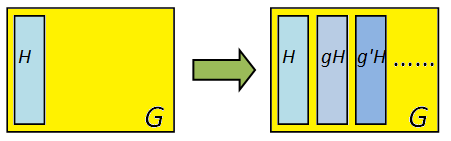
\includegraphics[scale=1]{figs/fig4.png}
\end{figure}
The union of $Ha_1, Ha_2,\ldots$ is $G$ (they are equivalence classes) and $Ha_i \cap Ha_j = \varnothing$ if $i\neq j$. For any $a_i$ we have $|H| = |Ha_i|$ since mapping $h$ to $ha_i$ is a bijection. \\

Thus $G$ is a disjoint union of $n=|G:H|$ cosets, each with size $|H|$. So we have $|G:H||H| = |G|$ and hence $\frac{|G|}{|H|}=|G:H|$ is an integer. In particular $|G|$ is a multiple of $|H|$.   
\end{proof}
The theorem immediately leads to the following 

\begin{coll}{}{}
If $G$ is finite group and $g\in G$ then $o(g)$ divides $G$
\end{coll}
\begin{proof}
Consider the subgroup $H=\ang{g}$ and we know that $|H| = o(g)$ the corollary follows immediately from  Lagrange's Theorem. 
\end{proof}

\begin{coll}{}{}
If $G$ is a finite group with $|G|=n$ then for all $g\in G$ we have $g^n = e$
\end{coll}
\begin{proof}
Let $g\in G$ and $k=o(g)$ divides $n$ by the above corollary. Thus $n=k\ell$ for integer $\ell$ then $g^n = g^{k\ell} = (g^k)^\ell = e^\ell = e$
\end{proof}
\newpage
\begin{coll}{}{}
If $|G|=p$ where $p$ is prime then every $G$ is cyclic. For any non-identity element we have $G=\ang{g}$
\end{coll}
\begin{proof}
Let $G$ be a group with $|G|=p$. Since $p\geq 2$ there is a non-identity element $g\in G$. We set $H=\ang{g}$. Then $|H|>1$ since the generator of $H$ has order larger than $1$. But $|H|$ must divide $|G|$ by Lagrange's Theorem. The only multiples of $|G|= p$ are $1$ and $p$ itself since $p$ is prime. Thus we must have $|H|=p= |G|$, so $H=G=\ang{g}$ showing $G$ is cyclic. 
\end{proof}


\newpage

\section{Introduction to Rings}

\begin{defn}{Ring}{}
A ring is a structure equipped with two binary operations denoted by addition $(+)$ and multiplication. With the following conditions 
\begin{itemize}
\item[\#1] The set $(R,+)$ is an abelian group. (The identity is denoted by $0$). 


\item[\#2] The set $(R,\cdot)$ is a monoid. (The identity of the monoid is denoted by $1$). 

\item[\#3] Left and right distributive laws hold. That is for all $a,b,c\in R$
\begin{align*}
a(b+c) &= ab+ac\\
(a+b)c &= ac+bc
\end{align*}
\end{itemize}
\end{defn}

If $\cdot$ is commutative then $R$ is called a \emph{commutative ring}. Some examples are:
\paragraph*{Example 1} The sets $\mathbb{Z,R,Q}$ with $\times, +$ are all commutative rings.  

\paragraph*{Example 2} For any positive integer $n$, the set of integers modulo $n$ $\mathbb{Z}/n\mathbb{Z}$. For the addition operation the previously defined addition will be used 
\[[a]+[b]=[a+b]\]
 
For the multiplication operation it is defined as follows 
\[[a]\cdot[b] = [ab]\]
Suppose we have $a,a^\prime, b,b^\prime$ such that $[a]=[a^\prime]$ and $[b]=[b^\prime]$. So we have $a-a' = kn$ and $b-b'=\ell n$ we want to show $[ab]=[a'b']$, so $ab-a'b'$ is a multiple of $n$. 
\[ab-a'b' = ab-ab'+ab'+a'b' = a(b-b')+b'(a-a')=a(\ell n) + b'(kn) = n(a\ell + b'k)\]
This proves that $ab\equiv a'b'\bmod n$ so $[ab]=[a'b']$. The identity is $[1]$ and  it is easy to check that this is commutative. We need to check for the distributive laws. 
\\
Let $[a],[b],[c] \in \mathbb{Z}/n\mathbb{Z}$. Then notice that 
\[[a]\cdot ([b]+[c]) = [a]\cdot ([b+c]) = [a(b+c)] = [ab+ac] = [ab]+[ac] = [a][b]+[a][c]\] 
Since $\cdot$ is commutative the other case would be symmetric. So $\mathbb{Z}/n\mathbb{Z}$ is a commutative ring. 

\newpage
\paragraph*{Example 3} Let $(G,+)$ be a group. We let $End(G)$ denote the set of homomorphism $G\rightarrow G$. This is called the set of \emph{\textbf{endomorphisms}} of $G$. We can define addition on this set as follows: 
\[(\phi+\psi)(g) = \phi(g) + \psi(g)\]
We can show this is closed 
\begin{align*}
(\phi+\psi)(g+h) &= \phi(g+h)+\psi(g+h)\\
&= \phi(g)+\phi(h) + \psi(g) + \psi(h) \\
&= (\phi(g)+\psi(g)) + (\phi(h) + \psi(h))\\
&= (\phi+\psi)(g) + (\phi + psi)(h)
\end{align*}
This uses the fact that $G$ is abelian. The identity element is the $\mathbf{0}:G\rightarrow G$ given by $\mathbf{0}(g) = 0$ since for any $\phi(g)$ we have $(\phi+\mathbf{0})(g) = \phi(g) + \mathbf{0}(g) = \phi(g)+0=\phi(g)$. For inverse the inverse is $-\phi(g)$. 
\[(\phi+(-\phi))(g)  = \phi(g)-\phi(g) = 0\]
For associativity consider $(\phi + \psi + \pi)(g)$
\[((\phi+\psi)(g) + \pi(g)) = (\phi(g)+\psi(g)+\pi(g))=(\phi(g)+(\psi+\pi)(g))\] 
Multiplication is defined as
\[\phi\psi = \phi\circ \phi\]
Since composition of homomorphism is a homomorphism we get $\phi\psi \in Eng(G)$ . The identity is given by $\iota(g) = g$. To check for distributive law consider: 
\begin{align*}
\phi(\psi+\pi)(g) &= \phi(\psi(g)+\pi(g))\\
&=\phi(\psi(g)) + \phi(\pi(g))\\
&=\phi\psi(g) + \phi\pi(g)\\
&=(\phi\psi+\phi\pi)(g)
\end{align*}


\newpage
\subsection{Properties of Rings and Definitions}

\begin{thm}{}{}
Let $0$ be the additive identity for any $a\in R$ we have 
\[a\cdot 0 = 0 = 0\cdot a\] 
\end{thm}
\begin{proof}
\begin{align*}
a\cdot 0 &= a\cdot (0+0) = a\cdot 0 + a\cdot 0\\
a\cdot 0 - a\cdot 0 &= a\cdot 0 + a\cdot 0 - a\cdot 0 \\
0 &= a\cdot 0
\end{align*}
Similar argument for $0\cdot a$ will apply. 
\end{proof}


\begin{thm}{}{}
Let $R$ be a ring and let $a,b\in R$ then 
\[(-a)b=a(-b) = -(ab)\]
\[(-a)(-b) = (ab)\]
\end{thm}
\begin{proof}
Since additive inverse of an element is unique we need show that both $a(-b)$ and $(-a)(b)$ are inverses of $(ab)$. 
\[(-a)(b) +(ab) = (-a+a)b = 0\cdot b = 0\]
The same argument will apply for $(a)(-b)$ thus by uniqueness of inverse $(-a)b=a(-b) = -(ab)$. 
\\
Now we can apply the first part to get
\[(-a)(-b) = -(a(-b))=-(-(ab)) = ab\]
\end{proof}

\begin{defn}{Characteristic of ring}{}
The characteristic of a ring denoted by $Char R$ is the order of multiplicative identity $1$ in the group under addition. If the order of $1$ is not finite then $Char R = 0$
\end{defn}
For the rings $\mathbb{Z,R,Q}$ all of them have characteristic 0. While any since there is no positive integer $n$ such that $n\cdot 1 = 0$.  For the ring $\mathbb{Z}/n\mathbb{Z}$ it has characteristic $n$ since $n[1] = [n] = [0]$. 

\newpage

\begin{thm}{}{}
If $Char(R) > 0$ then for $r\in R$ we have $k\cdot r = 0$ if and only if $n|k$. If $Char(R)= 0$ then $k\cdot r = 0$ if and only if $k=0$. 
\end{thm}
\begin{proof}
Suppose $n=Char(R)$ and let $k$ such that $n|k$. Let $r\in R$. We have $k=mn$ for some $m$. Then $(mn)\cdot r = ((mn)\cdot 1)\cdot r$ by distributivity.  Since we have $n\cdot 1 = 0$ we get 
\[r((mn)\cdot 1) = r(m(n\cdot 1)) = r(m\cdot 0) = r0 = 0\]

Now suppose $k$ is an integer such that for all $r\in R$ we have $r\cdot k = 0$. Then $k\cdot 1 = 0 = n\cdot 0$. So $R$ must be a multiple of $o(1)$ in the additive group. Using the \hyperref[thm5]{Theorem 5} for groups in additive notation we have $k=0\bmod n$ therefore $n|k$
\\
Finally, suppose $Char R = 0$ if $k=0$ then $0\cdot r = 0$. Conversely if $k\cdot r = 0$ then $k\cdot 1 = 0$ since $o(1)=\infty$ this only happens when $k=0$. 

\end{proof}


\section{Subrings and Homomorphisms}


\begin{defn}{Sub ring}{}
Let $R$ be a ring. $S$ is a subring of $R$, if addition and multiplication on $R$ restrict to binary operations on $S$, and $S$ is a ring with respect to those operations. Moreover
\[\mathbf{1}_R=\mathbf{1}_S\]
Their multiplicative identities are the same.  
\end{defn}

The following example shows why we needed the $1_R = 1_S$ condition. 

\paragraph{Example 1} Consider the Ring $\mathbb{Z}/6\mathbb{Z}$. The subset $S = \{[0],[2],[4]\}$ of even equivalence classes. $(S,+)$ is an abelian group moreover it is a cyclic group generated by $\ang{[2]}$. It is also closed under multiplication. Here $[4]$ acts as the identity for any $a\in S$ we have $4\times [a] = [a]$. But this is not a subring since $\mathbf{1}_\mathbb{Z}\neq \mathbf{1}_{\mathbb{Z}/n\mathbb{Z}}$.
\\

The set $\mathbb{Z}$ is a subring of $\mathbb{Q,R}$. It satisfies all the conditions and the multiplicative identity is same in all 2 sets. 

\newpage

\begin{thm}{Sub-Ring Test}{}
Let $S$ be a sub set of $(R,+, \times)$.  $S$ is a sub ring if the following conditions hold: 
\begin{itemize}
\item $1_R \in S$ 
\item if $a,b \in S$ then $a-b\in S$
\item if $a,b \in S$ then $ab\in S$. 
\end{itemize}
\end{thm}
\begin{proof}
Assume $S\subseteq R$ satisfies all the conditions. Then by the second condition $(S,+)$ is a group (Sub group test). Using the third condition $S,\times$ is closed under addition. Associatively holds because it held in $R$. Since we have $1_R \in S$ then $1_R\cdot s = s\cdot 1_R = s$ so by uniqueness of identity element $1_R = 1_S$. The distributive law holds since it holds in $R$.  
\\

Conversely assume $S$ is a sub ring of $R$. First since $(S,+)$ is a subgroup by the subgroup test the condition holds. Since $S$ is closed under multiplication the third condition holds. Finally we know that $1_S = 1_R$ so we must have $1_R\in S$ to the first condition holds as well. 


\end{proof}

\paragraph{Example 2} Center of a ring 

\subsection{Ring Homomorphisms}

\begin{defn}{Ring Homomorphism}{}
A function $\phi : R\rightarrow S$ for rings $S,R$ is called a \emph{ring homomorphism} if the following conditions hold: 
\begin{align}
\phi(a+b) &= \phi(a) + \phi(b)\\
\phi(ab) &= \phi(a)\phi(b) \\
\phi(\mathbf{1_R}) &= \mathbf{1_S}
\end{align}
\end{defn}

\subsection*{---------EXAMPLES------}

\newpage
\setcounter{equation}{0}

\begin{thm}{Properties of Ring homomorphisms}{}
Let $\phi: R_1 \rightarrow R_2$ be a ring homomorphism. Then the following hold: 
\begin{align}
\phi(0) &= 0 \\
\phi(-r) &= -\phi(r)\\
\phi(kr) &= k\phi(r) \text{ For $k\in \mathbb{Z}$} \\
\phi(r^n) &= \phi(r)^n \text{ For $n\in \mathbb{N}$} \\
\phi(r^k) &= \phi(r)^k \text{ For all $k\in \mathbb{Z}$ if $r$ is a \emph{unit}}
\end{align}


\end{thm}


\section{Ideals and Quotient Rings}

\subsection{Quotient Rings}

For defining quotient rings. We need to prove fundamental result about the relationship between kernels and normal subgroups. 
\begin{thm}{}{}
Let $G$ be a group
\begin{itemize}
\item[(1)] If $G_1$ is any group and $\phi: G\rightarrow G_1$ is a homomorphism then $\ker \phi$ is a normal subgroup of $G$. 
\item[(2)] If $H$ is a normal subgroup of $G$ then there is a group homomorphism $\phi: G\rightarrow G_1$ such that $H = \ker \phi$.  
\end{itemize}
\end{thm}
\begin{proof}
\begin{itemize}
\item[(1)] Suppose we have a homomorphism $\phi:G\rightarrow G_1$ and the set $K=\ker \phi$. We already know that $K$ is a subgroup of $G$. Suppose we have $h\in gKg^{-1}$ then $h = gkg^{-1}$ for some $k\in K$. Then we get
\[\phi(h) = \phi(gkg^{-1}) = \phi(g)\phi(k)\phi(g^{-1}) = \phi(g)e\phi(g^{-1}) = \phi(g)\phi(g)^{-1} = e\]
Therefore we have $h\in K$. So we know that $gKg^{-1}\subseteq K$. Taking $g^{-1}$ in place of $g$ we get $g^{-1}Kg \subseteq K$ this implies $K\subseteq gKg^{-1}$ hence we have $K = gKg^{-1}$ by definition $K=\ker \phi \lhd G$

\item[(2)] Suppose $H\lhd G$, let $G_1 = G/H$ and consider the quotient homomorphism $q:G\rightarrow G/H$ given by $q(g) = Hg$ we have $g\in \ker q$ if and only if $Hg = He$ that implies $e^{-1}g\in H$ that means we have $g\in H$. So we have $H=\ker q$
\end{itemize}
\end{proof}
This theorem shows that normal subgroups of $G$ same as the kernels of  homomorphisms of $G$.  

\newpage
\begin{defn}{Kernel of Rings}{}
Let $R,S$ be rings and let $\phi:R\rightarrow S$ be a group homomorphism the kernel is given by 
\[\ker \phi = \{r\in R : \phi(r) = 0_S\}\] 
\end{defn}
Since the way ring homomorphisms are constructed the kernel of a ring homomorphism with domain $R$ is automatically a additive subgroup of $R$.  

\subsection{Ideals}
\begin{defn}{Ideals}{}
Let $R$ be a ring. A subset $I$ of $R$ is called an ideal if 
\begin{itemize}
\item[\#1] $I$ is a subgroup of the additive group $R$. 
\item[\#2] $I$ \emph{absorbs} multiplication. That is, if $r\in I$ and $a\in R$, then $ra,ar\in I$. 
\end{itemize}
\end{defn}
\paragraph{Example 1} If $R$ is a ring then both $R$ and $\{0\}$ are ideals of $R$. The set $\{0\}$ is the trivial subgroup of $(R,+)$ and for any $r\in R$ we have $r\cdot 0 = 0\cdot r=0\in \{0\}$. This is called the \emph{zero ideal} of $R$. 

\paragraph{Example 2} For any $n\in \mathbb{N}$ the additive groups $n\mathbb{Z}$ are ideals of $\mathbb{Z}$. We know that $n\mathbb{Z}$ is a subgroup. To check for the absorption property, for any $m\in n\mathbb{Z}$ we have $m=nk$ it follows that 
\[\ell m = m\ell = (nk)\ell = n(k\ell) \in n\mathbb{Z}\]

\begin{thm}{}{}
Let $R$ be a ring and $I\subseteq R$ be an ideal. Then the set of right cosets $R/I$ can be given the structure of a ring with addition defined as $(I+a)+(I+b) = I+a+b$ and multiplication being $(I+a)(I+b) = I+ab$ 
\end{thm}
\begin{proof}
We know that $I$ is an additive group of $R$, since $(R,+)$ is an abelian group, every subgroup is normal and $R/I$ is also an abelian group.   
\\
Now we need to check that multiplication is well defined, suppose $a,b,a',b' \in R$ such that $I+a=I+a'$ and $I+b = I+b'$, this means that we have $a-a'\in I$ and $b-b'\in I$ we have to show that $I+ab = I+a'b'$ which means we have to show $ab-a'b' \in I$
\[ab-a'b' = ab-a'b+a'b-a'b' = (a-a')b + a'(b-b')\]
Since $a-a'\in I$ and it absorbs multiplication we have $(a-a')b\in I$ and same applies for $a'(b-b')\in I$. Finally $I$ is closed under addition so we get $ab-a'b' \in I$
\\
The element $I+1$ is the multiplicative identity since $(I+a)(I+1) = I+a\cdot 1 = I+a$ we can easily check that this operation is associative. Now for the distributive property
\begin{align*}
((I+a)+(I+b))(I+c) &= (I+a+b)(I+c)\\
&= (I+c(a+b))\\
&= I+ca+cb \\
&= (I+ca)+(I+cb)\\
&= (I+a)(I+c) + (I+b)(I+c)
\end{align*}
\end{proof}

The theorem connecting kernels with groups and normal subgroup  also holds for rings and ideals. 

\begin{thm}{}{}
Let $R$ be a ring
\begin{itemize}
\item[(1)] Let $S$ be any ring and $\phi:R\rightarrow S$ be a ring homomorphism then $\ker \phi$ is an ideal of $R$. 
\item[(2)] Let $I$ be an ideal of $R$ then there is a ring $R_1$ such that
$\phi:R\rightarrow R_1$ is a ring homomorphism and $I = \ker \phi$
\end{itemize}
\end{thm}
\begin{proof}
\begin{itemize}
\item[(1)] Let $K=\ker\phi$, $K$ is closed under multiplication since we have let $a \in K$ and $b\in R$ so we get $\phi(ab)=\phi(a)\phi(b) = 0_S\cdot 0_S$ therefore $ab\in K$ absorbs multiplication.  we already know that $K\lhd (R,+)$  so $I$ is an ideal. 

\item[(2)] Let $I$ be an ideal of $R$ consider the quotient mapping $q:R\rightarrow R/I$ given by $q(a) = I+a$, we can check by definition of the operations on $R/I$ that $q$ is a ring homomorphism.  Now let $a\in \ker q$ which means we have $q(a) = I+a = I+0$, which holds if $a\in I$ therefore $I=\ker q$

\end{itemize}
\end{proof}

\paragraph{Example} The sets $n\mathbb{Z}$ are ideals for the ring $\mathbb{Z}$ then the coset $n\mathbb{Z}+m$ corresponds to the equivalence class $[m]$ under congruence modulo $n$.   The multiplication 

\[(n\mathbb{Z}+m_1)(n\mathbb{Z}+m_2) = n\mathbb{Z}+m_1m_2\]
This corresponds to the multiplication $[m_1][m_2] = [m_1m_2]$ 












































































































 






















\end{document}
